\noindent
\begin{minipage}[t]{0.26\textwidth}
    \vspace*{9.5cm}
    \noindent
    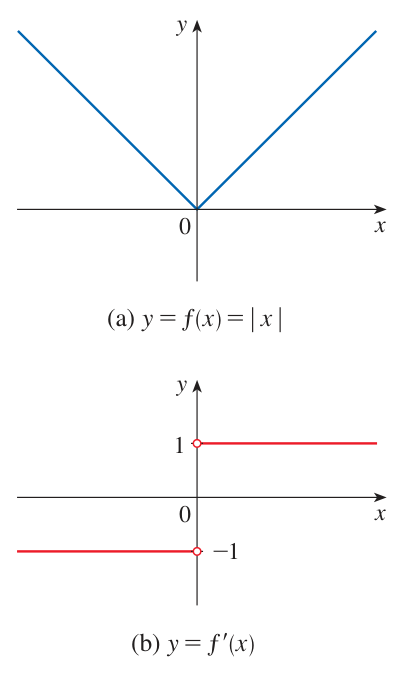
\includegraphics[width=\linewidth]{images/p0192_fig1.png}\\[5pt]
    \textbf{\textsf{HÌNH 5}}
\end{minipage}%
\hfill
\begin{minipage}[t]{0.70\textwidth}
    \noindent
    \textbf{\textsf{\color{stewartcyan}VÍ DỤ 5}}\quad Hàm số $f(x) = |x|$ khả vi tại những điểm nào?

    \vspace{0.6em}
    \noindent
    \textbf{\textsf{\color{stewartcyan}LỜI GIẢI}}\quad Nếu $x > 0$, thì $|x| = x$ và ta có thể chọn $h$ đủ nhỏ sao cho $x + h > 0$ và do đó $|x + h| = x + h$. Vì vậy, với $x > 0$, ta có
    \begin{align*}
        f'(x) &= \lim_{h \to 0} \frac{|x + h| - |x|}{h} = \lim_{h \to 0} \frac{(x + h) - x}{h} \\
        &= \lim_{h \to 0} \frac{h}{h} = \lim_{h \to 0} 1 = 1
    \end{align*}
    và do đó $f$ khả vi với mọi $x > 0$.

    \vspace{0.4em}
    Tương tự, với $x < 0$ ta có $|x| = -x$ và $h$ có thể được chọn đủ nhỏ sao cho $x + h < 0$ và vì thế $|x + h| = -(x + h)$. Do đó, với $x < 0$,
    \begin{align*}
        f'(x) &= \lim_{h \to 0} \frac{|x + h| - |x|}{h} = \lim_{h \to 0} \frac{-(x + h) - (-x)}{h} \\
        &= \lim_{h \to 0} \frac{-h}{h} = \lim_{h \to 0} (-1) = -1
    \end{align*}
    và do đó $f$ khả vi với mọi $x < 0$.

    \vspace{0.4em}
    Với $x = 0$, ta cần phải khảo sát
    \begin{align*}
        f'(0) &= \lim_{h \to 0} \frac{f(0 + h) - f(0)}{h} \\
        &= \lim_{h \to 0} \frac{|0 + h| - |0|}{h} = \lim_{h \to 0} \frac{|h|}{h} \qquad \text{(nếu tồn tại)}
    \end{align*}
    Hãy tính riêng rẽ các giới hạn trái và phải:
    \begin{alignat*}{2}
        &\lim_{h \to 0^+} \frac{|h|}{h} &&= \lim_{h \to 0^+} \frac{h}{h} = \lim_{h \to 0^+} 1 = 1 \\[4pt]
        \text{và}\qquad &\lim_{h \to 0^-} \frac{|h|}{h} &&= \lim_{h \to 0^-} \frac{-h}{h} = \lim_{h \to 0^-} (-1) = -1
    \end{alignat*}
    Vì các giới hạn này khác nhau nên $f'(0)$ không tồn tại. Do đó $f$ khả vi tại mọi $x$ ngoại trừ 0.

    \vspace{0.4em}
    Công thức của $f'$ được cho bởi
    \[
        f'(x) = \begin{cases}
            1 & \text{nếu } x > 0 \\[2pt]
            -1 & \text{nếu } x < 0
        \end{cases}
    \]
    và đồ thị của nó được thể hiện trong Hình~5(b). Việc $f'(0)$ không tồn tại được phản ánh về mặt hình học qua thực tế là đường cong $y = |x|$ không có tiếp tuyến tại $(0, 0)$. [Xem Hình~5(a).]\hfill{\color{stewartcyan}$\blacksquare$}

    \vspace{1.0em}
    Cả tính liên tục và tính khả vi đều là các tính chất mong muốn đối với một hàm số. Định lý sau đây cho thấy hai tính chất này có mối liên hệ với nhau như thế nào.

    \vspace{0.8em}
    \begin{tcolorbox}[
        colback=white,
        colframe=stewartred,
        boxrule=0.8pt,
        arc=0mm,
        left=8pt,
        right=8pt,
        top=7pt,
        bottom=7pt
    ]
        \noindent
        \tcbox[
            on line,
            colback=white,
            colframe=stewartred,
            boxrule=0.8pt,
            arc=1.5pt,
            top=1.5pt,
            bottom=1.5pt,
            left=4pt,
            right=4pt
        ]{\bfseries\color{stewartred}\textsf{4}}\hspace{8pt}%
        {\bfseries\color{stewartred}\textsf{Định lý}}\quad
        Nếu $f$ khả vi tại $a$, thì $f$ liên tục tại $a$.
    \end{tcolorbox}
\end{minipage}
